\documentclass[tikz, border=2pt]{standalone}
\usepackage{amsmath}

\begin{document}
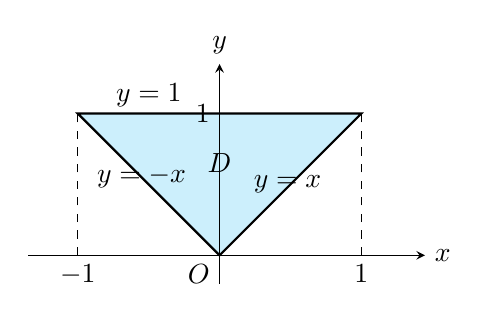
\begin{tikzpicture}[scale=1.8, >=stealth]
    % D: 0 <= y <= 1, -y <= x <= y
    \fill[cyan!20] (0,0) -- (-1,1) -- (1,1) -- cycle;

    \draw[->] (-1.35,0) -- (1.45,0) node[right] {$x$};
    \draw[->] (0,-0.2) -- (0,1.35) node[above] {$y$};

    \draw[thick] (0,0) -- (-1,1) -- (1,1) -- cycle;
    \draw[dashed] (-1,0) -- (-1,1);
    \draw[dashed] (1,0) -- (1,1);

    \node[below left] at (0,0) {$O$};
    \node[below] at (-1,0) {$-1$};
    \node[below] at (1,0) {$1$};
    \node[left] at (0,1) {$1$};
    \node at (0,0.65) {$D$};
    \node at (-0.55,0.55) {$y=-x$};
    \node at (0.48,0.5) {$y=x$};
    \node at (-0.5,1.13) {$y=1$};
\end{tikzpicture}
\end{document}
